\documentclass[a4paper]{article}

% \usepackage[default]{fontsetup}

\usepackage{fancyhdr}
\usepackage{extramarks}
\usepackage{amsmath}
\usepackage{amsthm}
\usepackage{amsfonts}
\usepackage{graphicx}
\usepackage{tikz}
\usepackage[plain]{algorithm}
\usepackage{algpseudocode}
\usepackage{enumerate}
\usepackage{tikz}

\usetikzlibrary{automata,positioning}

%
% Basic Document Settings
%  

\topmargin=-0.2in
\evensidemargin=0in
\oddsidemargin=0in
\textwidth=6.5in
\textheight=9.5in
\headsep=0.25in

\linespread{1.1}

\pagestyle{fancy}
\lhead{\hmwkAuthorName}
\chead{\hmwkClass : \hmwkTitle}
\rhead{\firstxmark}
\lfoot{\lastxmark}
\cfoot{\thepage}

\renewcommand\headrulewidth{0.4pt}
\renewcommand\footrulewidth{0.4pt}

\setlength\parindent{0pt}

%
% Create Problem Sections
%

\newcommand{\enterProblemHeader}[1]{
    \nobreak\extramarks{}{Problem \arabic{#1} continued on next page\ldots}\nobreak{}
    \nobreak\extramarks{Problem \arabic{#1} (continued)}{Problem \arabic{#1} continued on next page\ldots}\nobreak{}
}

\newcommand{\exitProblemHeader}[1]{
    \nobreak\extramarks{Problem \arabic{#1} (continued)}{Problem \arabic{#1} continued on next page\ldots}\nobreak{}
    \stepcounter{#1}
    \nobreak\extramarks{Problem \arabic{#1}}{}\nobreak{}
}

\newcommand*\circled[1]{\tikz[baseline=(char.base)]{
		\node[shape=circle,draw,inner sep=2pt] (char) {#1};}}


\setcounter{secnumdepth}{0}
\newcounter{partCounter}
\newcounter{homeworkProblemCounter}
\setcounter{homeworkProblemCounter}{1}
\nobreak\extramarks{Problem \arabic{homeworkProblemCounter}}{}\nobreak{}

%
% Homework Problem Environment
%
% This environment takes an optional argument. When given, it will adjust the
% problem counter. This is useful for when the problems given for your
% assignment aren't sequential. See the last 3 problems of this template for an
% example.
%

\newenvironment{homeworkProblem}[1][-1]{
    \ifnum#1>0
        \setcounter{homeworkProblemCounter}{#1}
    \fi
    \section{Problem \arabic{homeworkProblemCounter} (20\%)}
    \setcounter{partCounter}{1}
    \enterProblemHeader{homeworkProblemCounter}
}{
    \exitProblemHeader{homeworkProblemCounter}
}

%
% Homework Details
%   - Title
%   - Class
%   - Due date
%   - Name
%   - Student ID

\newcommand{\hmwkTitle}{Homework\ \#01}
\newcommand{\hmwkClass}{Probability \& Statistics for EECS}
\newcommand{\hmwkDueDate}{2024-10-6}
\newcommand{\hmwkAuthorName}{Zhang Yiheng}
\newcommand{\hmwkAuthorID}{2025531068}


%
% Title Page
%

\title{
    \vspace{2in}
    \textmd{\textbf{\hmwkClass:\\  \hmwkTitle}}\\
    \normalsize\vspace{0.1in}\small{Due\ on\ \hmwkDueDate\ at 23:59}\\
	\vspace{4in}
}

\author{
	Name: \textbf{\hmwkAuthorName} \\
	Student ID: \hmwkAuthorID}
\date{}

\renewcommand{\part}[1]{\textbf{\large Part \Alph{partCounter}}\stepcounter{partCounter}\\}

%
% Various Helper Commands
%

% Useful for algorithms
\newcommand{\alg}[1]{\textsc{\bfseries \footnotesize #1}}
% For derivatives
\newcommand{\deriv}[1]{\frac{\mathrm{d}}{\mathrm{d}x} (#1)}
% For partial derivatives
\newcommand{\pderiv}[2]{\frac{\partial}{\partial #1} (#2)}
% Integral dx
\newcommand{\dx}{\mathrm{d}x}
% Alias for the Solution section header
\newcommand{\solution}{\textbf{\large Solution}}
% Probability commands: Expectation, Variance, Covariance, Bias
\newcommand{\E}{\mathrm{E}}
\newcommand{\Var}{\mathrm{Var}}
\newcommand{\Cov}{\mathrm{Cov}}
\newcommand{\Bias}{\mathrm{Bias}}

\begin{document}


% \maketitle
% \thispagestyle{empty}
% \pagebreak

\date{
Due on Sep. 27, 2026, 23:59 UTC+8}
\title{SI 140A.02  Probability \& Statistics for EECS, Fall 2026 \\
Homework 1}
\maketitle
Read all the instructions below carefully before you start working on the assignment, and before you make a submission.
\begin{itemize}
    \item You are required to submit your homework in PDF format generated by \textbf{LaTeX}, otherwise you will get no points of this homework.
    \item You are required to write down all the major steps towards making your conclusions; otherwise you may obtain limited points of the problem.
    \item Write your homework in English; otherwise you will get no points of this homework.
    \item Any form of plagiarism will lead to $0$ point of this homework. 
\end{itemize}
\newpage

\begin{homeworkProblem}[1] 
\textbf{(Story Proof)}
Let \(S(n,k)\) denote the number of ways to partition
\(\{1,2,\ldots,n\}\) into \(k\) nonempty, unlabeled subsets.
Give a story proof for each of the following identities.

\begin{enumerate}
    \item[(a)] Prove that
    \[
        S(n+1,k)=S(n,k-1)+kS(n,k).
    \]

    \item[(b)] Prove that
    \[
        S(n,k)
        =
        \sum_{j=k-1}^{n-1}
        \binom{n-1}{j}S(j,k-1).
    \]
\end{enumerate}






\medskip
\solution

\begin{enumerate}
    \item[(a)]
    Consider the element \(n+1\). There are two possible cases.

    First, suppose that \(n+1\) is not in a block by itself. We first
    partition the other \(n\) elements into \(k\) nonempty blocks,
    which can be done in \(S(n,k)\) ways. We then insert \(n+1\) into
    one of these \(k\) blocks. Therefore, this case gives
    \(kS(n,k)\) partitions.

    Second, suppose that \(n+1\) forms a block by itself. The other
    \(n\) elements must then be partitioned into \(k-1\) nonempty
    blocks, which can be done in \(S(n,k-1)\) ways.

    Since the two cases are disjoint and include all possibilities,
    \[
        S(n+1,k)=S(n,k-1)+kS(n,k).
    \]

    \item[(b)]
    Fix the element \(n\) and consider the elements that are not in
    the same block as \(n\). There must be at least \(k-1\) such
    elements, since they have to form the other \(k-1\) nonempty
    blocks. There can be at most \(n-1\) such elements.

    Suppose exactly \(j\) elements are not in the same block as \(n\).
    These \(j\) elements can be selected from the other \(n-1\)
    elements in
    \[
        \binom{n-1}{j}
    \]
    ways. They can then be partitioned into \(k-1\) nonempty blocks
    in \(S(j,k-1)\) ways. The remaining \(n-1-j\) elements must be in
    the same block as \(n\). Thus, for a fixed \(j\), the number of
    possible partitions is
    \[
        \binom{n-1}{j}S(j,k-1).
    \]

    Summing over all possible values of \(j\), we obtain
    \[
        S(n,k)
        =
        \sum_{j=k-1}^{n-1}
        \binom{n-1}{j}S(j,k-1).
    \]
\end{enumerate}





\end{homeworkProblem}
\newpage
\begin{homeworkProblem}[2]

A \emph{nonrepeat password} is a nonempty sequence formed from
\(m\) distinct symbols, where no symbol may appear more than once.
The length of the password is \(\ell\) which could be any integer from \(1\) to \(m\).
Suppose that one password is chosen uniformly at random from all
nonrepeat passwords.

Let \(p_m\) be the probability that the selected password uses all
\(m\) symbols.

\begin{enumerate}
    \item[(a)] Find an expression for \(p_m\).

    \item[(b)] Show that
    \[
        p_m
        =
        \frac{1}{
        \displaystyle\sum_{j=0}^{m-1}\frac{1}{j!}
        }
        \text{ and }
        \lim_{m\to\infty}p_m=\frac{1}{e},
    \]

    where \(e\) is the base of the natural logarithm.
\end{enumerate}

\medskip
\solution

\begin{enumerate}
    \item[(a)]
    If the password has length \(\ell\), we first choose \(\ell\)
    symbols from the \(m\) distinct symbols and then arrange them.
    Thus, there are \(\binom{m}{\ell}\ell!\) passwords of length
    \(\ell\). Since \(1\leq\ell\leq m\), the total number of
    nonrepeat passwords is
    \[
        \sum_{\ell=1}^{m}\binom{m}{\ell}\ell!.
    \]
    There are \(m!\) passwords that use all \(m\) symbols. Because
    every password is equally likely,
    \[
        p_m
        =\frac{m!}
        {\displaystyle\sum_{\ell=1}^{m}\binom{m}{\ell}\ell!}.
    \]

    \item[(b)]
    Using \(\binom{m}{j}j!=m!/(m-j)!\), we obtain
    
    \[
    p_m
    =\frac{m!}{\sum_{j=1}^{m}\binom{m}{j}j!}
    =\frac{1}{\sum_{j=1}^{m}1/(m-j)!}
    =\frac{1}{\sum_{j=0}^{m-1}1/j!}.
    \]

    It remains to show that
    \[
        \lim_{m\to\infty}\sum_{j=0}^{m-1}\frac{1}{j!}=e.
    \]
    By the binomial theorem,
    \[
        \left(1+\frac{1}{n}\right)^n
        =\sum_{k=0}^{n}\binom{n}{k}\frac{1}{n^k}.
    \]
    For each fixed \(k\),
    \[
        \binom{n}{k}\frac{1}{n^k}
        =\frac{1}{k!}
          \prod_{r=0}^{k-1}\left(1-\frac{r}{n}\right)
        \longrightarrow \frac{1}{k!}
        \qquad (n\to\infty).
    \]
    Moreover,
    \[
        0\leq\binom{n}{k}\frac{1}{n^k}\leq\frac{1}{k!}.
    \]
    The tails of \(\sum_{k=0}^{\infty}1/k!\) tend to zero, so this
    bound allows us to pass the limit through the sum. Since
    \(\lim_{n\to\infty}(1+1/n)^n=e\), it follows that
    \[
        e=\sum_{k=0}^{\infty}\frac{1}{k!}
        =\lim_{m\to\infty}\sum_{j=0}^{m-1}\frac{1}{j!}.
    \]
    Therefore,
    \[
        \lim_{m\to\infty}p_m=\frac{1}{e}.
    \]
\end{enumerate}

\end{homeworkProblem}

\newpage
\begin{homeworkProblem}[3]
\textbf{(Geometry Probability)}
    You get a stick and break it randomly into three pieces. Two breaking points are chosen independently and uniformly.
What is the probability that you can make a triangle using such three pieces?

\medskip
\solution

Let the stick have length \(l\), and let two of the three pieces have
lengths \(x\) and \(y\). The third piece has length \(l-x-y\).
The sample space is
\[
    \Omega=\{(x,y):x>0,\ y>0,\ x+y<l\}.
\]
Because the two breaking points are chosen independently and uniformly,
\((x,y)\) is uniformly distributed over this triangular region.

The three pieces form a triangle exactly when each piece is shorter
than \(l/2\). Thus the valid region is
\[
    T=\{(x,y):x<l/2,\ y<l/2,\ x+y>l/2\}.
\]

\begin{center}
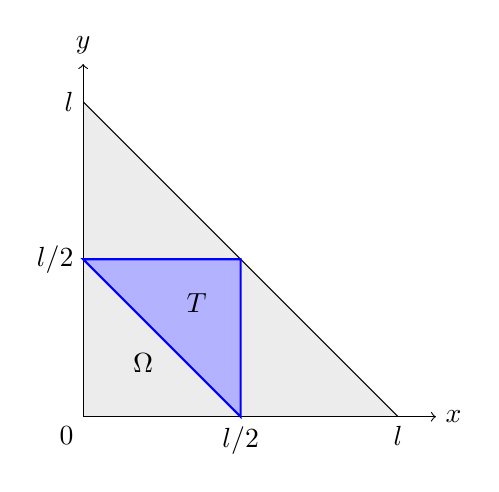
\begin{tikzpicture}[scale=4]
    \fill[gray!15] (0,0) -- (1,0) -- (0,1) -- cycle;
    \fill[blue!30] (0,.5) -- (.5,0) -- (.5,.5) -- cycle;

    \draw[->] (0,0) -- (1.12,0) node[right] {\(x\)};
    \draw[->] (0,0) -- (0,1.12) node[above] {\(y\)};
    \draw (1,0) -- (0,1);
    \draw[thick,blue] (0,.5) -- (.5,0) -- (.5,.5) -- cycle;

    \node[below left] at (0,0) {\(0\)};
    \node[below] at (.5,0) {\(l/2\)};
    \node[below] at (1,0) {\(l\)};
    \node[left] at (0,.5) {\(l/2\)};
    \node[left] at (0,1) {\(l\)};
    \node at (.19,.17) {\(\Omega\)};
    \node at (.36,.36) {\(T\)};
\end{tikzpicture}
\end{center}

Both regions are right triangles. The legs of \(\Omega\) have length
\(l\), while the legs of \(T\) have length \(l/2\). Therefore,
\[
    P(\text{the pieces form a triangle})
    =\frac{\operatorname{Area}(T)}{\operatorname{Area}(\Omega)}
    =\frac{\frac12(l/2)^2}{\frac12l^2}
    =\boxed{\frac14}.
\]

\end{homeworkProblem}


\newpage
\begin{homeworkProblem}[4]
\textbf{(Birthday Problem)}
In the birthday problem, we assumed that all 365 days of the year are equally likely (and excluded February 29). In reality, some days are slightly more likely as birthdays than others. For example, scientists have long struggled to understand why more babies are born 9 months after a holiday. Let $\mathbf{p}=\left(p_1, p_2, \ldots, p_{365}\right)$ be the vector of birthday probabilities, with $p_j$ the probability of being born on the $j$ th day of the year (February 29 is still excluded, with no offense intended to Leap Dayers). The $k$ th elementary symmetric polynomial in the variables $x_1, \ldots, x_n$ is defined by
$$
e_k\left(x_1, \ldots, x_n\right)=\sum_{1 \leq j_1<j_2<\cdots<j_k \leq n} x_{j_1} \ldots x_{j_k},  \quad 2 \leq k \leq 365.
$$
This just says to add up all of the $\left(\begin{array}{l}n \\ k\end{array}\right)$ terms we can get by choosing and multiplying $k$ of the variables. For example, $e_1\left(x_1, x_2, x_3\right)=x_1+x_2+x_3, e_2\left(x_1, x_2, x_3\right)=x_1 x_2+$ $x_1 x_3+x_2 x_3$, and $e_3\left(x_1, x_2, x_3\right)=x_1 x_2 x_3$ Now let $k \geq 2$ be the number of people.\\
(a) Find a simple expression for the probability that there is at least one birthday match, in terms of $\mathbf{p}$ and an elementary symmetric polynomial.\\
(b) Explain intuitively why it makes sense that $P$ (at least one birthday match) is minimized when $p_j=\frac{1}{365}$ for all $j$, by considering simple and extreme cases.\\
(c) The famous arithmetic mean-geometric mean inequality says that for $x, y \geq 0$
$$
\frac{x+y}{2} \geq \sqrt{x y} .
$$
This inequality follows from adding $4 x y$ to both sides of $x^2-2 x y+y^2=(x-y)^2 \geq 0$ Define $\mathbf{r}=\left(r_1, \ldots, r_{365}\right)$ by $r_1=r_2=\left(p_1+p_2\right) / 2, r_j=p_j$ for $3 \leq j \leq 365$. Using the arithmetic mean-geometric mean bound and the fact, which you should verify, that
$$
e_k\left(x_1, \ldots, x_n\right)=x_1 x_2 e_{k-2}\left(x_3, \ldots, x_n\right)+\left(x_1+x_2\right) e_{k-1}\left(x_3, \ldots, x_n\right)+e_k\left(x_3, \ldots, x_n\right)
$$
show that

\begin{center}
    $P($ at least one birthday match $\mid \mathbf{p}) \geq P($ at least one birthday match $\mid \mathbf{r})$
\end{center}

with strict inequality if $\mathbf{p} \neq \mathbf{r}$, where the given $\mathbf{r}$ notation means that the birthday probabilities are given by $\mathbf{r}$. Using this, show that the value of $\mathbf{p}$ that minimizes the probability of at least one birthday match is given by $p_j=\frac{1}{365}$ for all $j$.



\newpage
\solution

\begin{enumerate}
    \item[(a)]
    To have no birthday match, the \(k\) people must have \(k\)
    distinct birthdays. For each choice of \(k\) distinct days,
    there are \(k!\) ways to assign them to the \(k\) people. Hence
    \[
        P(\text{at least one match}\mid\mathbf p)
        =1-k!e_k(p_1,\ldots,p_{365}).
    \]

    \item[(b)]
    Consider two simple cases. When \(k=2\), the probability of a
    match is \(\sum_{j=1}^{365}p_j^2\). Averaging two unequal
    probabilities decreases the sum of their squares, so the
    uniform distribution gives the smallest match probability.

    When \(k=365\), the probability of no match is
    \(365!\prod_{j=1}^{365}p_j\). By the arithmetic mean-geometric
    mean inequality, this product is largest when all the
    \(p_j\)'s are equal. At the other extreme, if everyone is born
    on the same day, a match is certain. These cases suggest that
    making birthdays more evenly distributed reduces the chance
    of a match.

    \item[(c)]
    In the definition of \(e_k\), each term contains either both
    \(x_1,x_2\), exactly one of them, or neither of them. These
    three disjoint cases give
    \[
    \begin{aligned}
        e_k(x_1,\ldots,x_n)
        ={}&x_1x_2e_{k-2}(x_3,\ldots,x_n)\\
          &+(x_1+x_2)e_{k-1}(x_3,\ldots,x_n)
            +e_k(x_3,\ldots,x_n).
    \end{aligned}
    \]

    Averaging \(p_1\) and \(p_2\) leaves their sum unchanged, so
    only the first term changes. In fact,
    \[
        e_k(\mathbf r)-e_k(\mathbf p)
        =\left(\frac{(p_1+p_2)^2}{4}-p_1p_2\right)
          e_{k-2}(p_3,\ldots,p_{365})
        =\frac{(p_1-p_2)^2}{4}
          e_{k-2}(p_3,\ldots,p_{365})
        \geq 0.
    \]
    Therefore,
    \[
        P(\text{at least one match}\mid\mathbf p)
        \geq
        P(\text{at least one match}\mid\mathbf r).
    \]
    The inequality is strict if \(p_1\ne p_2\) and
    \(e_{k-2}(p_3,\ldots,p_{365})>0\).

    Finally, let \(2\leq k\leq365\). Since \(e_k\) is continuous on
    the compact probability simplex, it attains a maximum. The uniform
    vector gives \(e_k=\binom{365}{k}(1/365)^k>0\), whereas any vector
    with fewer than \(k\) positive entries gives \(e_k=0\).
    Thus a maximizing vector must have at least \(k\) positive entries.
    After removing any two entries, at least \(k-2\) positive entries
    remain, so \(e_{k-2}\) of the remaining entries is positive
    (with the convention \(e_0=1\)). Assuming that two of its entries are
    unequal, averaging them would strictly increase \(e_k\) by
    the argument above, which leads to a contradiction. Thus all entries must
    be equal. 
    Consequently, the uniform vector minimizes the probability
    of at least one birthday match.
\end{enumerate}



\end{homeworkProblem}

\newpage

\begin{homeworkProblem}[5]

A card collection contains five different types of cards. Each
independent draw produces card type \(i\) with probability \(p_i\),
where
\[
    (p_1,p_2,p_3,p_4,p_5)
    =
    (0.05,0.15,0.20,0.25,0.35).
\]

Let \(Q_n\) denote the probability of collecting all five card types
after \(n\) independent draws. $n \geq 1$.

For each \(i\in\{1,\ldots,5\}\), define
\[
    E_i
    =
    \{\text{card type \(i\) does not appear in the first \(n\) draws}\}.
\]

For any index set
\[
    I\subseteq\{1,\ldots,5\},
\]
define
\[
    E_I=\bigcap_{i\in I}E_i.
\]
Thus, \(E_I\) is the event that none of the card types whose indices
belong to \(I\) appears in the first \(n\) draws. By convention,
\[
    E_{\emptyset}=\Omega,
\]
where \(\Omega\) denotes the entire sample space.

\begin{enumerate}
    \item[(a)]
    Use the inclusion-exclusion principle to prove that
    \[
        Q_n
        =
        \sum_{I\subseteq\{1,\ldots,5\}}
        (-1)^{|I|}
        \left(
        1-\sum_{i\in I}p_i
        \right)^n,
    \]
    where \(|I|\) denotes the number of elements in \(I\).

    \item[(b)]
    Find the smallest integer \(n\) such that $Q_n\geq 0.90.$ You can write some code to calculate it. Include the screenshot of your code and output in the terminal which can support your answer.

    \item[(c)]
    Find the smallest n for which the probability of collecting all five types is at least 0.90 in the uniform case. (No need to include the code)
    Write code to plot $Q_n$ as a function of $n$ for both equal and unequal $p_i$, along with their corresponding probabilities.  (You should incluide the graph.) 
    Compare \(Q_n\) with the corresponding probability between the two cases.
\end{enumerate}



\medskip
\solution

\begin{enumerate}
    \item[(a)]
    Collecting all five card types is the complement of the event
    \(E_1\cup\cdots\cup E_5\), which means that at least one type
    is missing. For any \(I\subseteq\{1,\ldots,5\}\), each draw avoids
    every type in \(I\) with probability
    \(1-\sum_{i\in I}p_i\). Since the draws are independent,
    \[
        P(E_I)=\left(1-\sum_{i\in I}p_i\right)^n.
    \]
    Applying the inclusion-exclusion principle to
    \(E_1\cup\cdots\cup E_5\) and then taking the complement gives
    \[
        Q_n
        =\sum_{I\subseteq\{1,\ldots,5\}}
          (-1)^{|I|}
          \left(1-\sum_{i\in I}p_i\right)^n.
    \]
    The term for \(I=\emptyset\) equals \(1\), as required.

    \item[(b)]
    Evaluating the inclusion-exclusion formula gives
    \(Q_{45}\approx 0.899893<0.90\) and
    \(Q_{46}\approx 0.904965\geq 0.90\).
    Since \(Q_n\) is nondecreasing in \(n\), the smallest integer
    satisfying \(Q_n\geq 0.90\) is \(\boxed{46}\).
    The code and its terminal output are shown below. Both views
    are cropped from the same screenshot.

    \begin{center}
        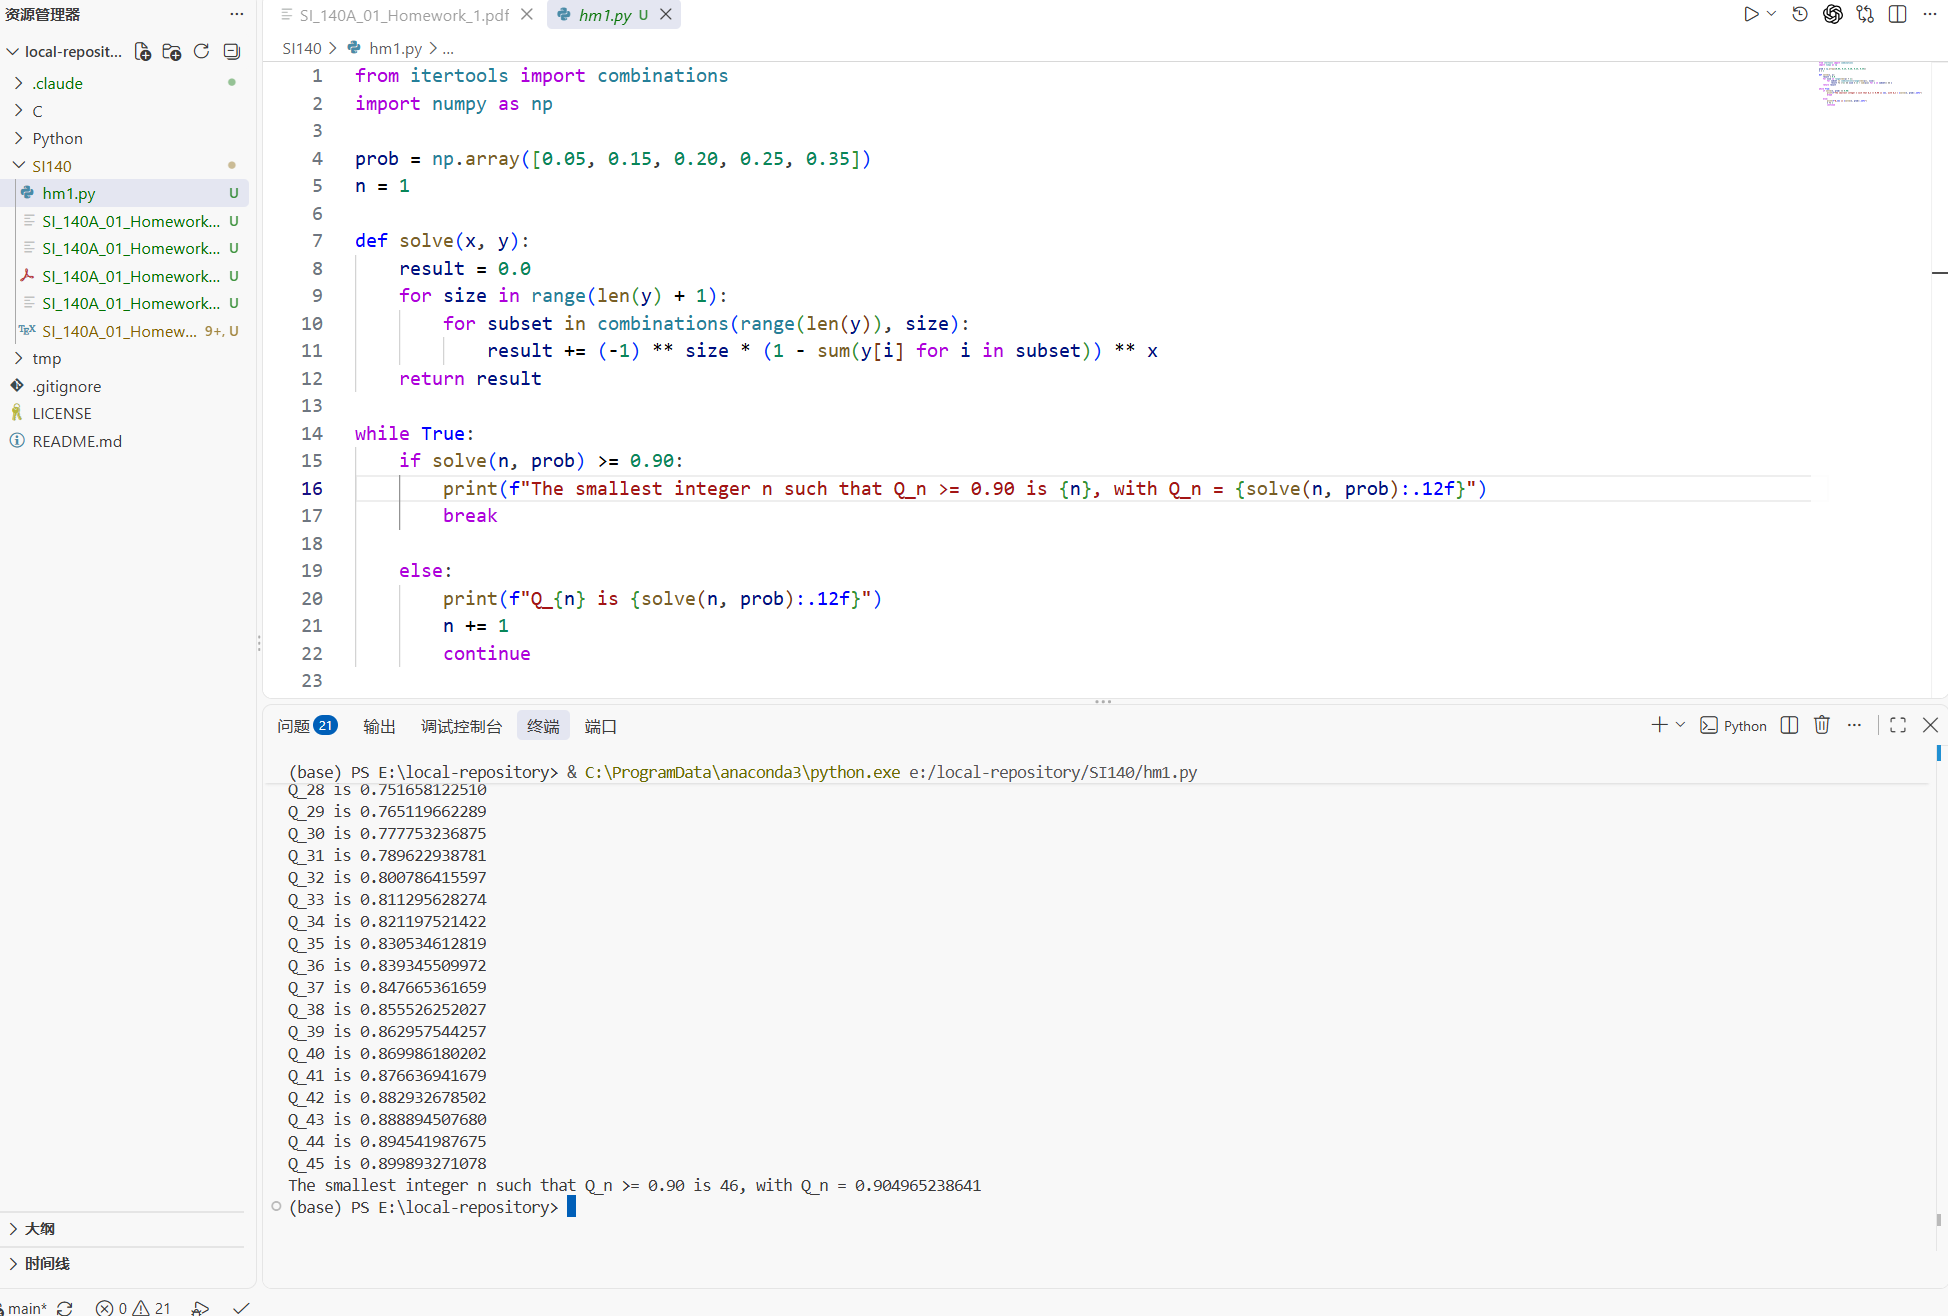
\includegraphics[width=\linewidth,
            trim=248bp 473bp 344bp 45bp,clip]{image1.png}

        \medskip
        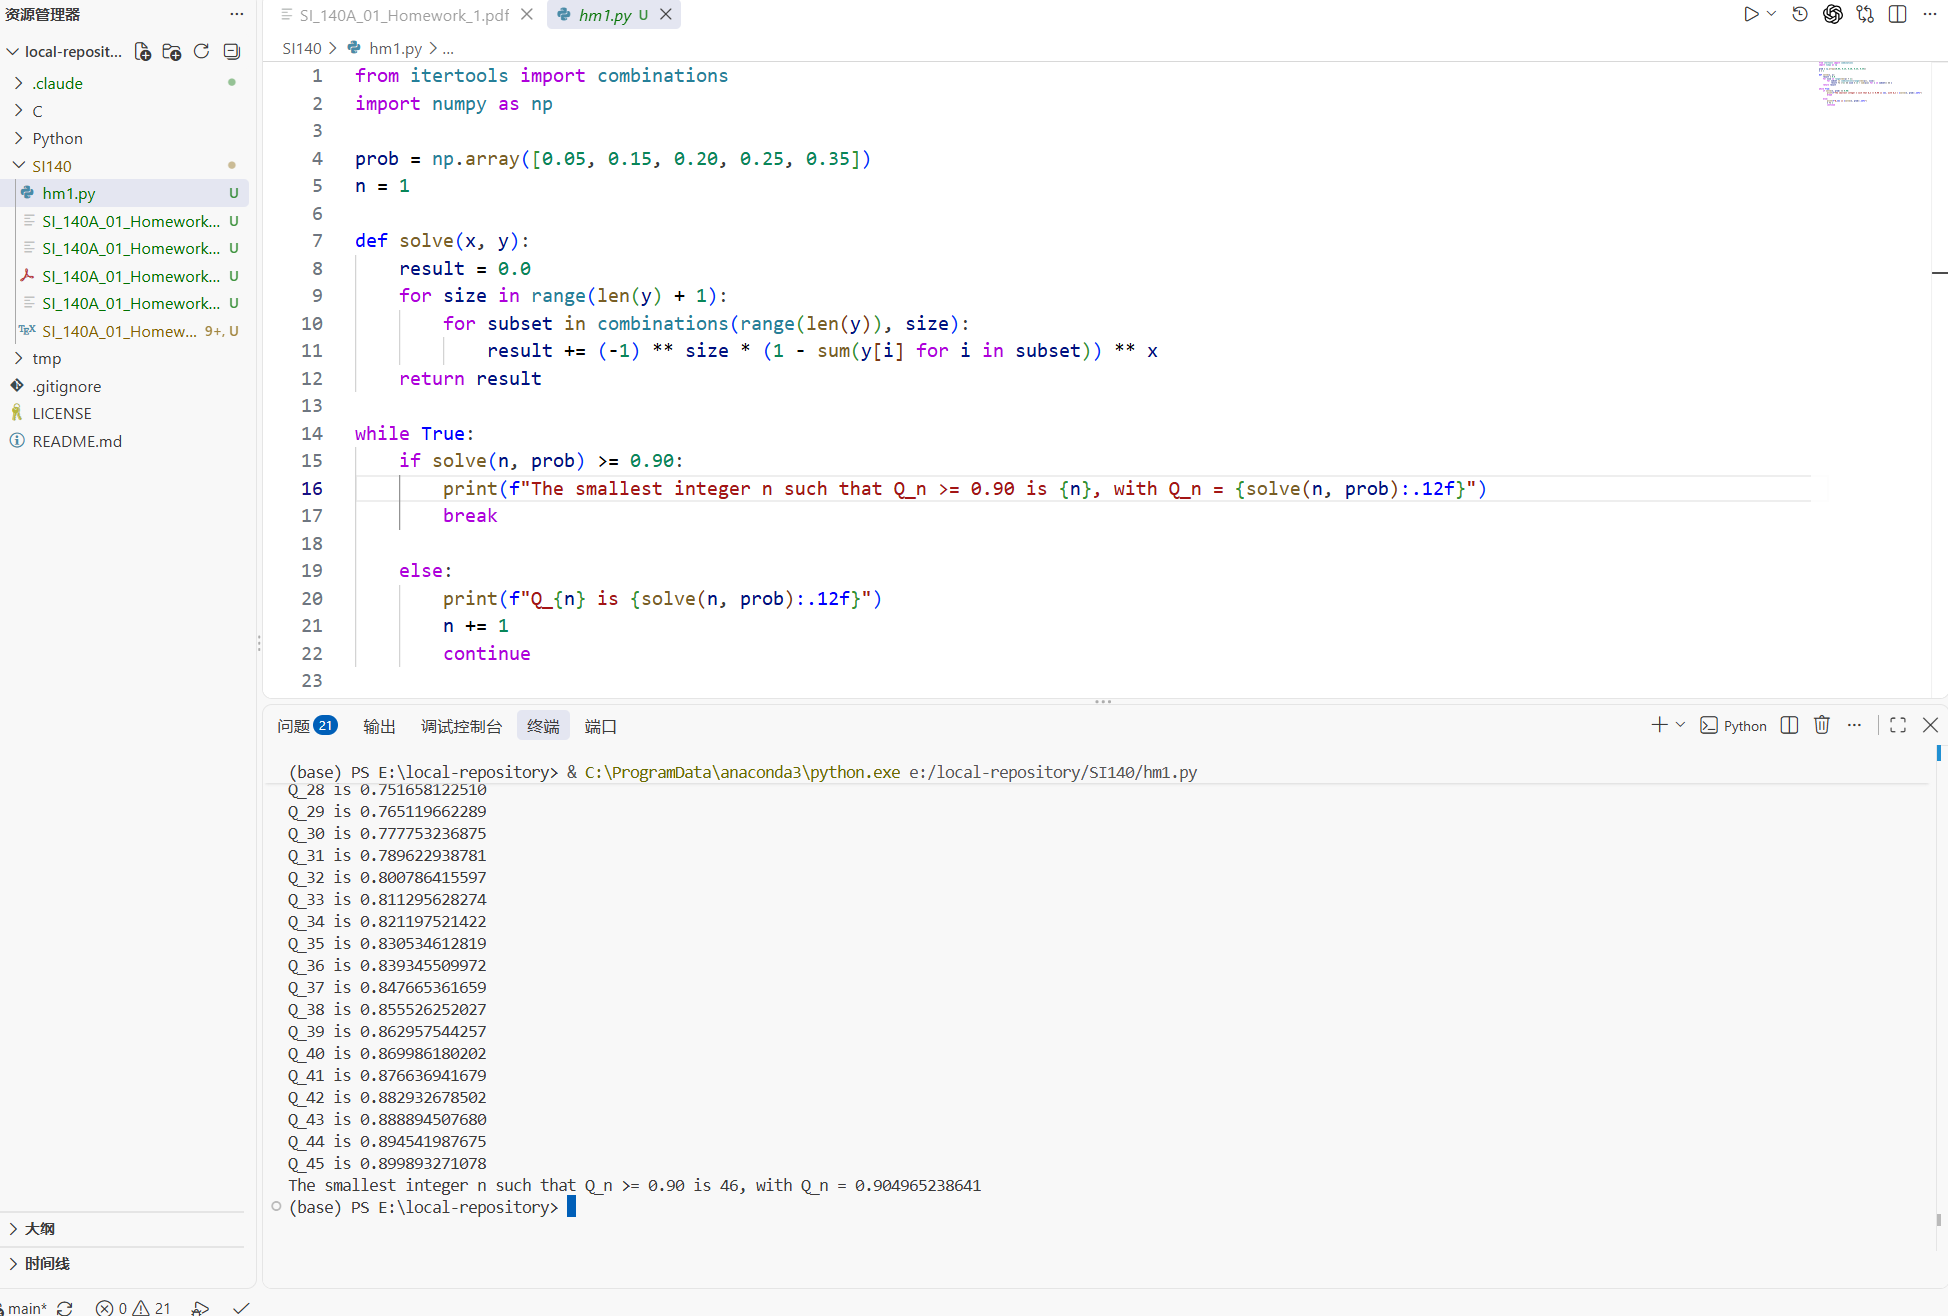
\includegraphics[width=\linewidth,
            trim=195bp 72bp 561bp 525bp,clip]{image1.png}
    \end{center}

    \newpage
    \item[(c)]
    In the uniform case, each card type has probability \(1/5\), so
    inclusion-exclusion simplifies to
    \[
        Q_n^{\mathrm{uniform}}
        =\sum_{j=0}^{5}(-1)^j\binom{5}{j}
          \left(1-\frac{j}{5}\right)^n.
    \]
    The computed values are \(Q_{17}^{\mathrm{uniform}}\approx0.889101<0.90\)
    and \(Q_{18}^{\mathrm{uniform}}\approx0.910943\geq0.90\).
    Hence the smallest \(n\) in the uniform case is \(\boxed{18}\).
    At \(n=18\), the unequal case has \(Q_{18}\approx0.550869\),
    much lower than the uniform case. The graph shows that the
    uniform probabilities reach the 0.90 target 28 draws earlier.

    \begin{center}
        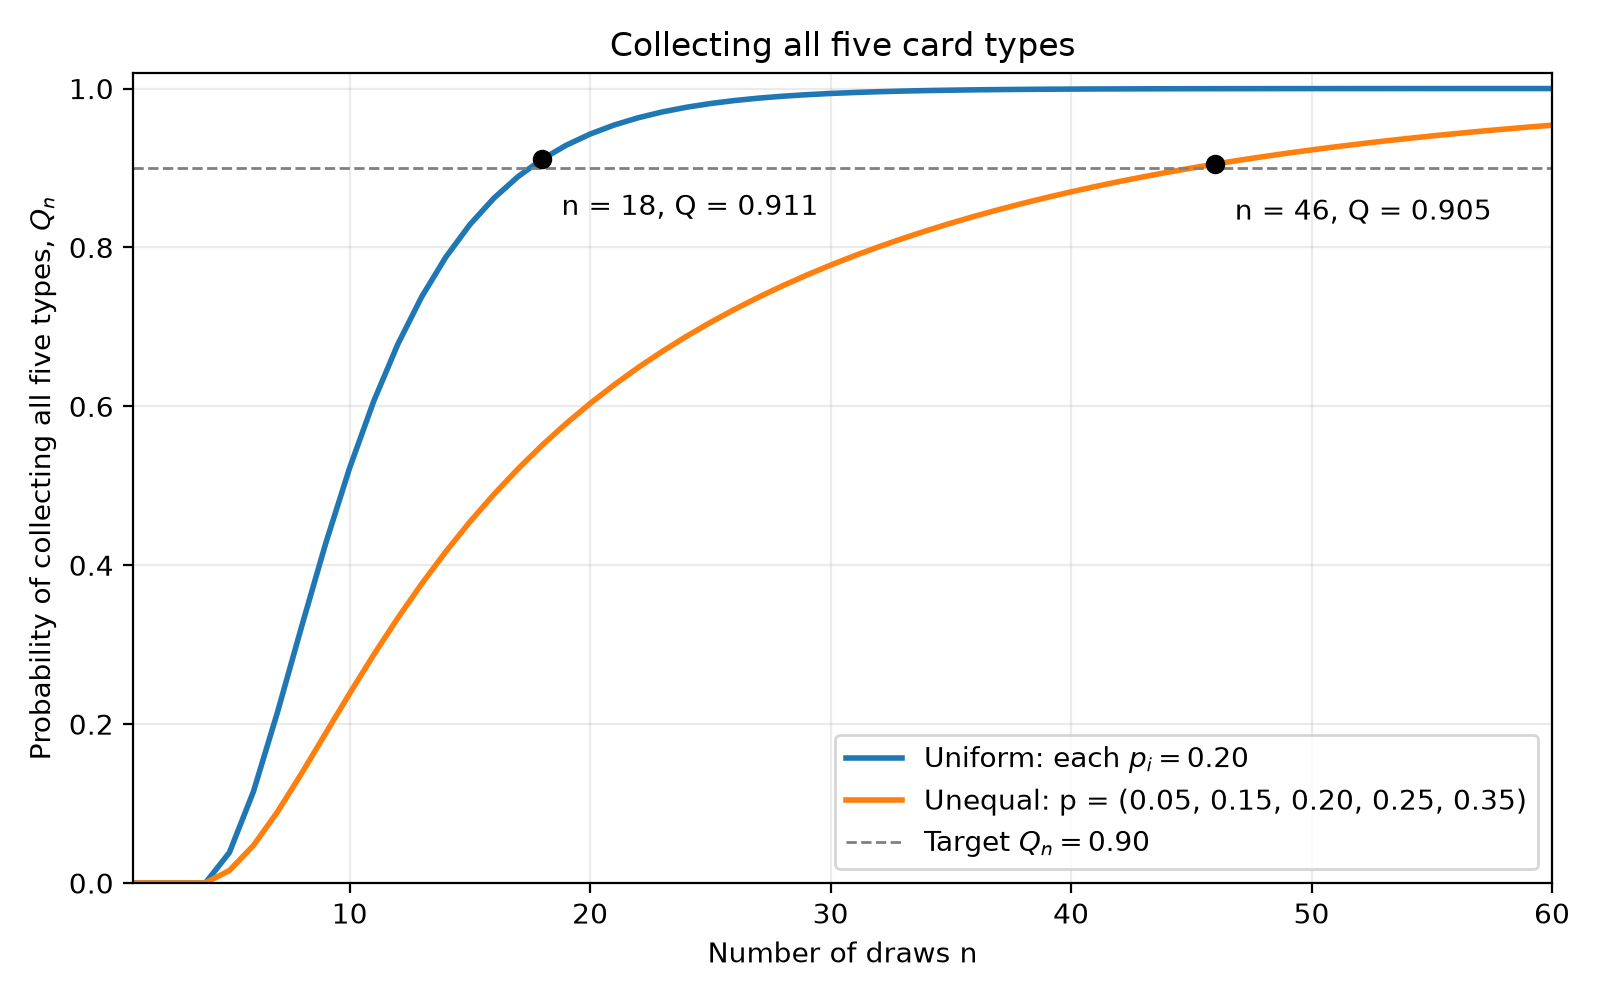
\includegraphics[width=\linewidth]{hm2_plot.png}
    \end{center}
\end{enumerate}



\end{homeworkProblem}

\end{document}
